\chapter{Architectural Design}
\label{chap:archdesign}

% Give block diagram showing the major components of your translator
% Describe the interfaces between the components
% State who implemented each component



% NOTE: I'd love for this image to have text wrap around it, but
%       I can't figure out how... :(
\begin{figure}
\begin{center}
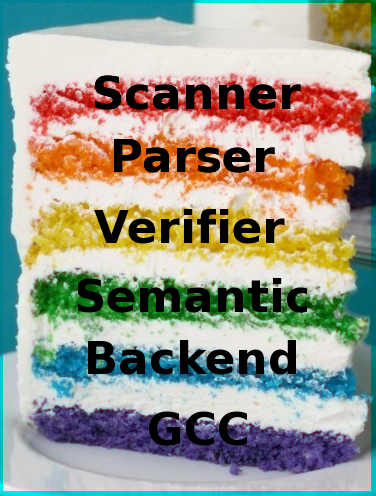
\includegraphics[width=60mm]{figures/layers.png}
\caption{A diagram showing the layers of \sys{}. The raw source code is
fed into the top of the cake and binary executables come out the bottom.}
\label{fig:layers}
\end{center}
\end{figure}

Our design incorporates six layers: the scanner, the parser, the verifier,
the semantic converter, the backend C generation, and C image manipulation
libraries (see Figure~\ref{fig:layers}). The compiler takes as input
a text file containing a valid \sys{} program and outputs a binary that
implements the program described by the input text.

The scanner generates as its output a one-dimensional list of
tokens (see Figure~\ref{fig:tokens}).

\begin{figure}[h]
\begin{center}
\begin{tabular}{l l l l l l l}

    SEMI & LPAREN & RPAREN & LTCHAR & GTCHAR & LBRKT & RBRKT \\
    LBRACE & RBRACE COLON & COMMA & FSLASH & CONVOP & PIPE \\
    ATSYM & UMINUS & UPLUS & ASSIGN & DEFINE & OREQUAL & IMAGET \\
    KERNELT & CALCT & CHANNELT & UINT8T & UINT16T & UINT32T & INT8T \\
    INT16T & INT32T & ANGLET & IMGREAD & IMGWRITE & LITSTR & CSTR \\
    INTEGER & ID & EOF \\

\end{tabular}
\caption{A comprehensive list of tokens produced by the lexical analysis
(scanner).}
\end{center}
\label{fig:tokens}
\end{figure}

The parser reads this token list and uses our context-free grammar to generate
an abstract syntax tree. The parser is not strict about which nodes have
which children, or whether or not it is meaningful to have the current
structure: rather it just blindly assembles the tree. The abstract syntax tree
has the nodes described in Figure~\ref{fig:astnodes}.

\begin{figure}
\begin{center}
\begin{tabular}{l | l}
{\bf Node} & {\bf Description} \\
\hline \\
stmt & Statement \\
vdecl & Variable Declaration \\
expr & Expression \\
matrix & Calc matrix \\
bareint & Integer \\
kerncalc & Kernel calculation \\
chanref & Image channel reference \\
libfunc & \sys{} library function \\
assign\_op & Assignment operation \\
atom & Atomic type
\end{tabular}
\caption{A list of abstract syntax tree nodes.}
\label{fig:astnodes}
\end{center}
\end{figure}

The verifier accepts as input an abstract syntax tree. It traverses the
tree and checks that nodes are arranged in meaningful ways. While it
traverses, it also builds up an environment that keeps track of all
variables defined, along with their identifier name and type. If the
verifier accepts the AST, it will return as output the cumulative
environment that contains the identifiers and their types.

The semantic converter takes in a verified abstract syntax tree and also the
list of variables generated by the verifier. It then maps each node or
configuration of nodes to a corresponding Semantic AST node that
corresponds more directly with the eventual C code that must be generated.
The output of this layer is a semantically checked abstract syntax tree
(SAST). The semantic converter also supplements the environment information
inherited from the verifier with additional information not related to
verification, such the largest referenced command-line argument.

% TODO: Mapping of AST -> SAST ??

The backend takes as input the SAST and the supplemented environment
information. It then converts this into a meaningful C++ program source
file. This program can be submitted to GCC and compiled.

The final layer of \sys{} is the GCC compiler. The generated C source from
the backend is fed into the GCC compiler, which outputs a binary in
architecture-specific assembly language.

The lead developers for each layer of \sys{} are identified in
Figure~\ref{fig:leads}.


\begin{figure}
\begin{center}
\begin{tabular}{l | l}
{\bf Layer} & {\bf Lead Developer} \\
\hline \\
Unit Tests & Kevin and Yongxu \\
Scanner & Jeremy \\
Parser & Jeremy \\
Verifier & Jeremy \\
Semantic & Robert \\
Backend & Robert \\
GCC & Richard Stallman et al. \\
\end{tabular}
\caption{Who Did What: The lead developer of each layer.}
\end{center}
\label{fig:leads}
\end{figure}


